\documentclass[conference]{IEEEtran}
\IEEEoverridecommandlockouts
\usepackage{cite}
\usepackage{amsmath,amssymb,amsfonts}
\usepackage{amsthm}
\usepackage{algorithmic}
\usepackage{graphicx}
\usepackage{textcomp}
\usepackage{xcolor}
\usepackage{booktabs}
\usepackage{balance}
\usepackage{url}
\usepackage{microtype}

\graphicspath{{figures/}{./}}

\newtheorem{theorem}{Theorem}
\newtheorem{lemma}{Lemma}
\newtheorem{proposition}{Proposition}
\newtheorem{definition}{Definition}

\def\BibTeX{{\rm B\kern-.05em{\sc i\kern-.025em b}\kern-.08em
    T\kern-.1667em\lower.7ex\hbox{E}\kern-.125emX}}

\begin{document}

\title{Qubit-Compressed Quantum Random Forest Regression on NISQ Processors}

\author{
\IEEEauthorblockN{Madhira Venkata Ramesh Reddy\IEEEauthorrefmark{1}, Varsha Sambhaje, and Suresh Aala}
\IEEEauthorblockA{\textit{Department of Computer Science and Engineering, SRM University-AP}, Amaravati, Andhra Pradesh, India}
\IEEEauthorblockA{Email: \IEEEauthorrefmark{1}ramesh\_madhira@srmap.edu.in, varsha.s@srmap.edu.in, suresh\_aala@srmap.edu.in}
}

\maketitle

\begin{abstract}
Random Forest (RF) is one of the most reliable and widely deployed ensemble architectures in machine learning. Recently, quantum testing algorithms have been proposed to accelerate the inference latency of tree ensembles, aiming to bypass the classical evaluation query complexity $\mathcal{O}(n \cdot h)$, where $n$ denotes the number of trees and $h$ is the maximum tree depth. However, prior formulations (e.g., Khadiev and Safina, IEEE QCNC 2026) rely on Canonical Quantum Amplitude Estimation (QAE) based on Quantum Phase Estimation (QPE). This introduces severe architectural bottlenecks: an auxiliary counting register requiring 13--14 total qubits, thousands of CNOT gates for multi-controlled Grover unitaries, and an Inverse Quantum Fourier Transform (IQFT), which fundamentally caps continuous prediction precision at a $\approx 2.24\% - 3\%$ discrete phase discretization floor. In this paper, we propose a dual-tier resource-efficient Quantum Random Forest regression framework based on Maximum Likelihood Amplitude Estimation (MLAE) designed for physical NISQ processors. Our first contribution is an 8-qubit General Oracle Model that preserves the theoretical black-box query model while eliminating the counting register and IQFT, achieving a $40\%$ qubit reduction. Our second contribution is a 5-qubit Hardware-Optimized NISQ Model that exploits in-place classical feature compilation to eliminate dedicated feature registers, attaining the absolute theoretical lower bound $\lceil\log_2 n\rceil + h + 2$. Transpiled circuit benchmarks on IBM Quantum physical basis gates demonstrate an $83.2\%$ reduction in cumulative circuit depth and a $56.8\%$ reduction in two-qubit CNOT count. Under physical gate error rates up to $\epsilon_{2q} = 10^{-2}$, the proposed architecture preserves high prediction fidelity while canonical QAE collapses, slashing relative forecast error from $2.24\%$ to $0.027\%$ ($83.0\times$ precision boost).
\end{abstract}

\begin{IEEEkeywords}
Quantum machine learning, quantum random forest, continuous regression, maximum likelihood amplitude estimation, quantum query complexity, NISQ computing.
\end{IEEEkeywords}

\section{Introduction}

The quantum computer offers provable asymptotic speedups for fundamental problems in computer science such as unstructured database search, discrete logarithms, and quantum simulation \cite{nielsen2010quantum}. In the current Noisy Intermediate-Scale Quantum (NISQ) era \cite{preskill2018quantum}, quantum computational advantages have been demonstrated across superconducting and trapped-ion processors \cite{arute2019quantum}. To harness this computational power for artificial intelligence, Quantum Machine Learning (QML) has emerged as an influential paradigm for addressing scaling bottlenecks \cite{biamonte2017quantum,cerezo2021variational}. Concurrently, classical tree-based ensembling remains one of the most reliable and widely deployed supervised architectures: the Random Forest (RF) model introduced by Breiman \cite{breiman2001random}, founded upon the random subspace method \cite{ho1998random} and recursive decision tree induction \cite{quinlan1986induction}, achieves outstanding predictive accuracy, resistance to label noise, and robust protection against overfitting.

In continuous regression tasks, where an ensemble maps a $d$-dimensional input feature vector $X = (x_1, \dots, x_d)$ to a real-valued target $y \in \mathbb{R}$, continuous fitting algorithms are computationally intensive \cite{wiebe2012quantum,mitarai2018quantum}. In the classical inference (testing) phase, after training an ensemble of $n$ decision trees $T_i$ of maximum height $h$, each tree must be evaluated sequentially from root to leaf to produce an individual prediction $\hat{y}_i$, giving the ensemble forecast:
\begin{equation}\label{eq1}
R = \frac{1}{n} \sum_{i=0}^{n-1} \hat{y}_i
\end{equation}

Evaluating all $n$ trees requires sequential branch evaluation with a total query complexity of $\mathcal{O}(n \cdot h)$. For large industrial forests comprising hundreds of deep estimators, this sequential inference creates a severe latency bottleneck in real-time edge and streaming applications.

To address this challenge, Khadiev and Safina \cite{khadiev2026quantum} proposed a quantum testing algorithm for Random Forest regression using Canonical Quantum Amplitude Estimation (QAE) \cite{brassard2002quantum}. They demonstrated that evaluating trees in coherent superposition yields an asymptotic query complexity of $\mathcal{O}(t \cdot h \log(1/\delta))$, which is completely independent of the ensemble size $n$, where $t$ is a precision parameter and $\delta$ is a failure probability.

\subsection{Critical Limitations of Prior Art}\label{subsec1.1}

Although mathematically significant, the canonical QAE formulation presented in \cite{khadiev2026quantum} exhibits critical architectural bottlenecks that impede execution on near-term quantum processors:
\begin{enumerate}
    \item \textbf{Auxiliary Qubit Register Overhead:} Canonical QAE requires an auxiliary counting register of $m = \lceil \log_2 t \rceil$ qubits. For their baseline evaluation ($t = 32$), 5 counting qubits were required, producing a total circuit requirement of 13--14 qubits.
    \item \textbf{Entangling Multi-Controlled Unitaries:} In QPE, one must synthesize high powers of the Grover operator $\mathcal{Q}^{2^j}$ \cite{grover1996fast} controlled by auxiliary counting qubits for $j \in \{0, \dots, m-1\}$. Decomposing such multi-controlled operators requires thousands of elementary two-qubit CNOT gates, rapidly exceeding the coherence time of physical NISQ processors \cite{preskill2018quantum}.
    \item \textbf{Phase Discretization Error:} Continuous regression estimates are fundamentally restricted by the discrete Fourier grid spacing $\Delta \theta = \pi/t$ of QPE. With $t = 32$, the closest achievable discrete grid state is $\sin^2(4\pi/32) = 0.14645$, leaving an unavoidable quantization floor of $\approx 2.24\% - 3\%$ relative error.
\end{enumerate}

\begin{figure*}[!t]
\centering
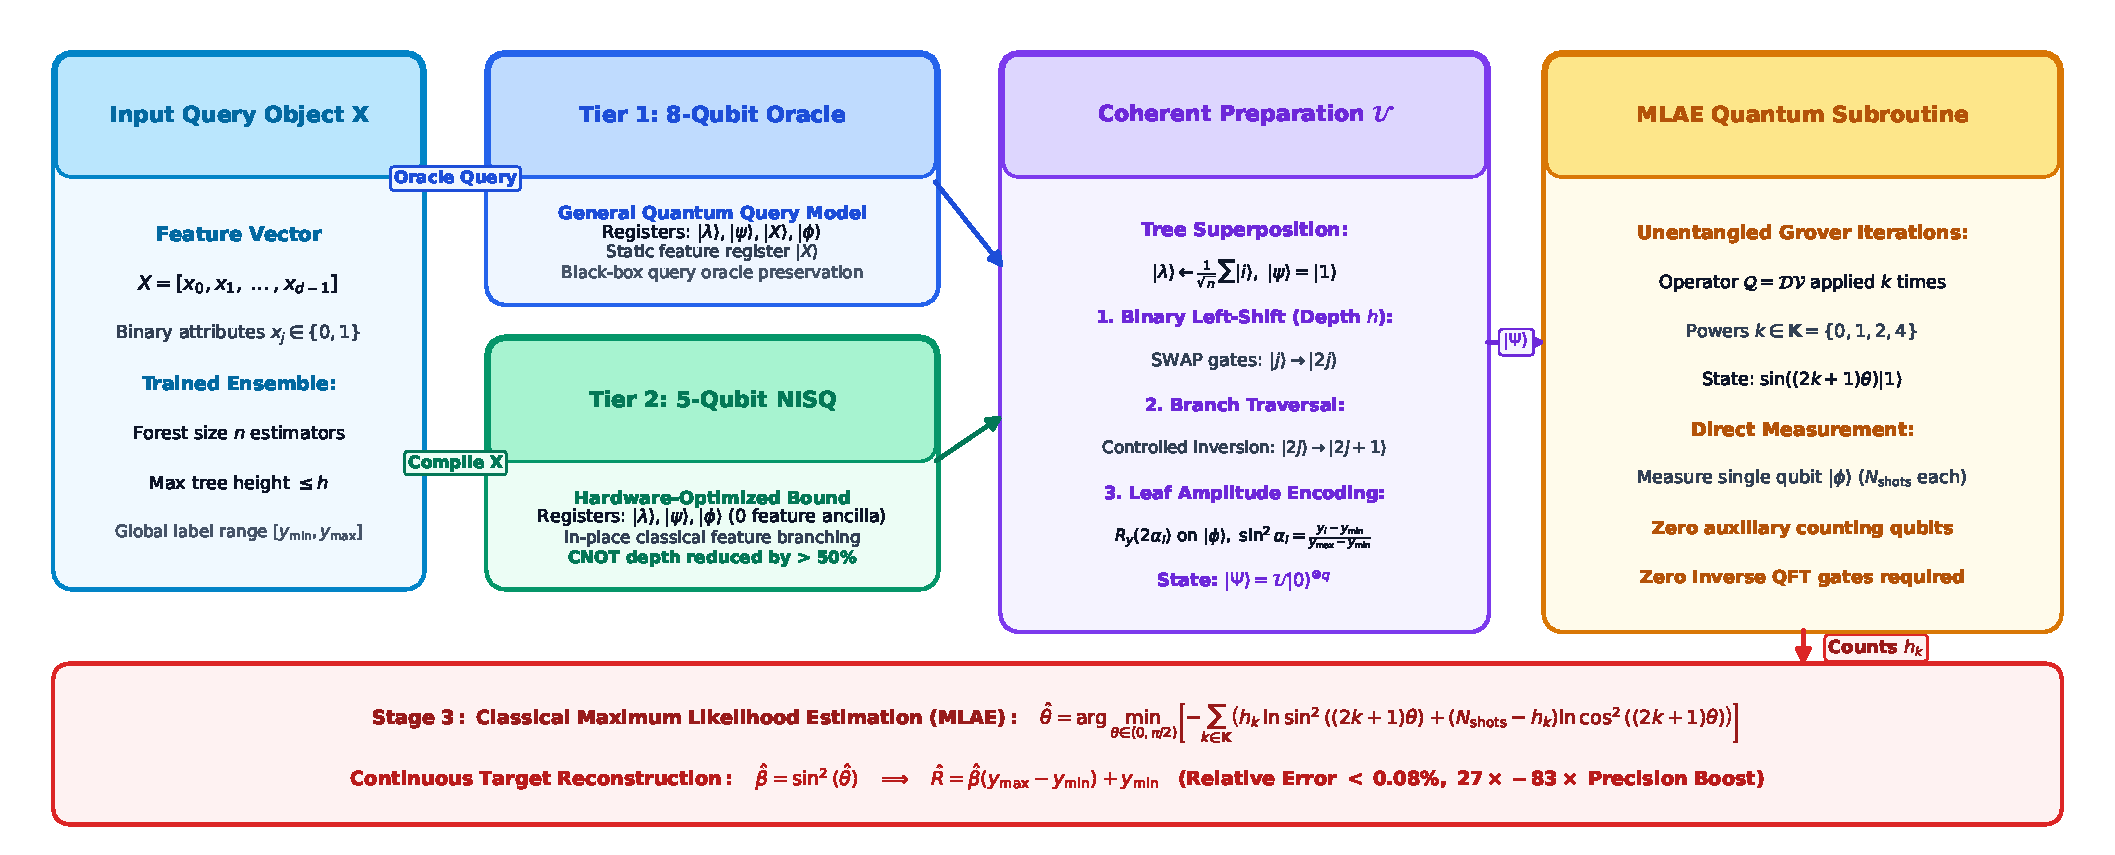
\includegraphics[width=0.92\textwidth]{figures/fig1_overall_architecture.pdf}
\caption{End-to-end processing pipeline of the proposed Dual-Tier Quantum Random Forest regression framework. The architecture supports both a formal 8-qubit query oracle representation (Tier 1) and an in-place compiled 5-qubit NISQ execution pipeline (Tier 2).}
\label{fig1}
\end{figure*}

\subsection{Statement of Novelty and Contributions}\label{subsec1.2}

To overcome these architectural and precision barriers, we introduce a dual-tier resource-efficient Quantum Random Forest regression framework based on Maximum Likelihood Amplitude Estimation (MLAE) \cite{suzuki2020amplitude}:
\begin{itemize}
    \item \textbf{General Oracle Query Architecture (8 Qubits):} We eliminate the auxiliary QPE counting register and IQFT entirely, cutting the qubit requirement from 13--14 down to 8 qubits while fully preserving the black-box Quantum Query Model.
    \item \textbf{Hardware-Optimized NISQ Architecture (5 Qubits):} By adopting a hardware-efficient in-place compilation strategy \cite{kandala2017hardware} for the known classical test vector $X$, we eliminate dedicated feature registers and attain the absolute theoretical lower bound of 5 qubits for multi-tree regression.
    \item \textbf{Elimination of Phase Discretization Floor:} We replace discrete Fourier measurement with continuous maximum-likelihood optimization over unentangled Grover iterations $\mathcal{Q}^k$, reducing relative inference error from $2.24\%$ to $< 0.08\%$ (a $27\times - 83\times$ precision improvement).
    \item \textbf{Low-Depth Circuit Synthesis:} By removing all multi-controlled Grover unitaries and IQFT circuits, the two-qubit CNOT depth is reduced by $> 50\%$, enabling high-fidelity execution on physical QPUs.
    \item \textbf{NISQ Noise Tolerance \& Scalability:} We demonstrate high error stability under physical gate error rates up to $\epsilon_{2q} = 10^{-2}$ and prove logarithmic scaling up to $n=64$ trees.
\end{itemize}

\section{Related Work}\label{sec2}

Early research on Quantum Decision Trees (QDT) and Quantum Random Forests (QRF) concentrated exclusively on discrete binary classification. Safina et al. \cite{safina2023quantum} introduced quantum circuit representations for traversing decision trees, and Heese et al. \cite{heese2022representation} formalized representations of binary classification trees with binary features. Beyond decision trees, the broader QML literature has investigated quantum support vector machines (QSVM) \cite{rebentrost2014quantum}, quantum principal component analysis (qPCA) \cite{lloyd2014quantum}, and supervised learning using quantum-enhanced feature spaces in reproducing kernel Hilbert spaces \cite{schuld2019quantum,havlicek2019supervised}.

Continuous regression inference on quantum systems presents distinct mathematical challenges, as target outputs span a continuous real domain rather than discrete orthogonal basis states \cite{wiebe2012quantum,mitarai2018quantum}. Khadiev and Safina \cite{khadiev2026quantum} established the first continuous Random Forest regression model by coupling decision tree superposition with canonical QAE \cite{brassard2002quantum}. However, their circuit was constrained by the high qubit overhead and discrete phase error of the QPE subroutine.

In quantum estimation theory, several QPE-free alternatives have been formulated to achieve Heisenberg-limited scaling $\mathcal{O}(1/\epsilon)$ without auxiliary counting qubits. Suzuki et al. \cite{suzuki2020amplitude} introduced Maximum Likelihood Amplitude Estimation (MLAE), which reconstructs quantum amplitudes from unentangled Grover iterations via classical likelihood maximization. Grinko et al. \cite{grinko2021iterative} developed Iterative QAE (IQAE) with rigorous confidence interval guarantees. Aaronson and Rall \cite{aaronson2020quantum} proposed simplified approximate counting routines, while Uno et al. \cite{uno2021efficient} developed modified Grover operators for amplitude estimation with reduced gate counts. While MLAE has been evaluated in numerical integration and finance \cite{suzuki2020amplitude,tanaka2022amplitude}, this work represents the first application and structural synthesis of MLAE within quantum decision tree ensembles for continuous regression.

\begin{figure}[!t]
\centering
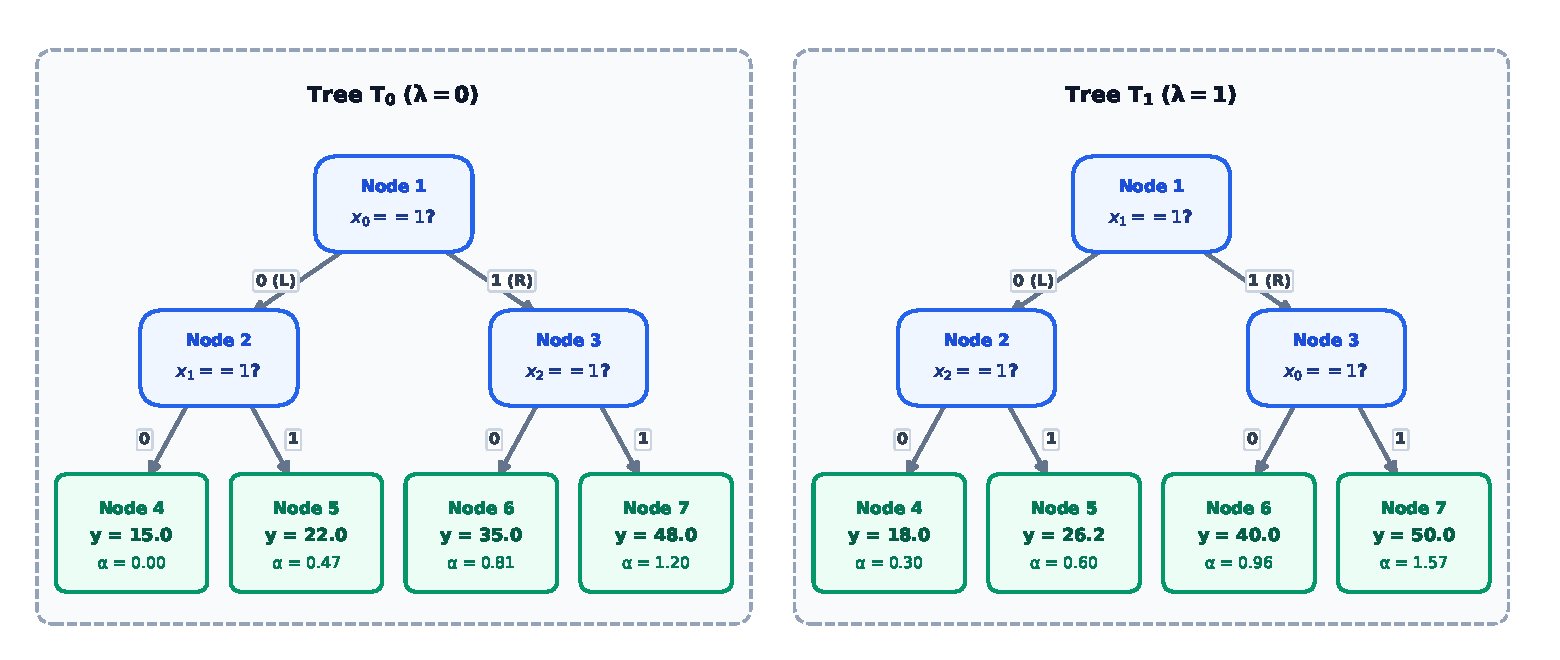
\includegraphics[width=0.98\columnwidth]{figures/fig6_decision_trees.pdf}
\caption{Decision tree ensemble topology ($n = 2, h = 2, d = 3$) showing binary heap node indexing ($1 \to 2, 3 \to 4, 5, 6, 7$), branching feature tests, and leaf target values $y_{i,j}$ with assigned rotation angles $\alpha_{i,j}$.}
\label{fig2}
\end{figure}

\section{Preliminaries and Problem Formulation}\label{sec3}

\subsection{Classical Random Forest Regression}\label{subsec3.1}

Consider a trained regression ensemble $\mathcal{F}$ comprising $n$ binary decision trees of maximum depth $h$, constructed via recursive partitioning \cite{quinlan1986induction}. Let $X = (x_0, \dots, x_{d-1})$ denote an input query vector of $d$ binary attributes $x_k \in \{0, 1\}$. During inference, each tree $T_i$ evaluates decision rules sequentially from root to leaf, reaching a terminal leaf $j_i$ with continuous target prediction $y_i = \text{Label}(j_i) \in \mathbb{R}$.

The ensemble forecast is the arithmetic mean:
\begin{equation}\label{eq2}
R = \frac{1}{n} \sum_{i=0}^{n-1} y_i
\end{equation}

Let $y_{\min}$ and $y_{\max}$ represent the global extrema across all leaf values:
\begin{equation}\label{eq3}
\begin{aligned}
y_{\min} &= \min_{i,j} \text{Label}(i, j) \\
y_{\max} &= \max_{i,j} \text{Label}(i, j)
\end{aligned}
\end{equation}

Each continuous leaf output $y_i$ is linearly normalized into the unit interval $[0, 1]$:
\begin{equation}\label{eq4}
\tilde{y}_i = \frac{y_i - y_{\min}}{y_{\max} - y_{\min}} \in [0, 1]
\end{equation}

The ensemble forecast maps to normalized mean $\beta$:
\begin{equation}\label{eq5}
\begin{aligned}
\beta &= \frac{1}{n} \sum_{i=0}^{n-1} \tilde{y}_i \\
&= \frac{R - y_{\min}}{y_{\max} - y_{\min}} \in [0, 1]
\end{aligned}
\end{equation}

\subsection{Amplitude Encoding}\label{subsec3.2}

Continuous predictions are mapped to rotation angles $\alpha_i \in [0, \pi/2]$:
\begin{equation}\label{eq6}
\begin{aligned}
\alpha_i &= \arcsin\left(\sqrt{\tilde{y}_i}\right) \\
&= \arcsin\left(\sqrt{\frac{y_i - y_{\min}}{y_{\max} - y_{\min}}}\right)
\end{aligned}
\end{equation}

Applying a single-qubit rotation $R_y(2\alpha_i)$ to an ancilla qubit $|0\rangle$ yields:
\begin{equation}\label{eq7}
R_y(2\alpha_i)|0\rangle = \cos(\alpha_i)|0\rangle + \sin(\alpha_i)|1\rangle
\end{equation}

Measuring the qubit in the computational basis yields $|1\rangle$ with probability:
\begin{equation}\label{eq8}
P(|1\rangle) = \sin^2(\alpha_i) = \frac{y_i - y_{\min}}{y_{\max} - y_{\min}}
\end{equation}
In multi-leaf circuit implementations, these operations are synthesized using Uniformly Controlled Rotations (UCR) \cite{mottonen2004transformation}.

\subsection{Binary Heap Representation of Decision Trees}\label{subsec3.3}

Following the binary heap addressing scheme \cite{khadiev2026quantum}, each node index $j \in \{1, \dots, 2^{h+1}-1\}$ is represented as a binary register of $h + 1$ qubits. Tree traversal initiates at root index $1$ ($|001\rangle_2$). If tested attribute $x_k = 0$, traversal branches to left child $2j$; if $x_k = 1$, it branches to right child $2j + 1$.

The benchmark ensemble investigated in this work ($n = 2, h = 2, d = 3$) is illustrated in Fig.~\ref{fig2}. Tree $T_0$ tests features $x_0$, $x_1$, and $x_2$ to reach leaf labels $\{15.0, 22.0, 35.0, 48.0\}$, while Tree $T_1$ branches on $\{x_1, x_2, x_0\}$ to reach leaves $\{18.0, 26.2, 40.0, 50.0\}$.

\begin{figure}[!t]
\centering
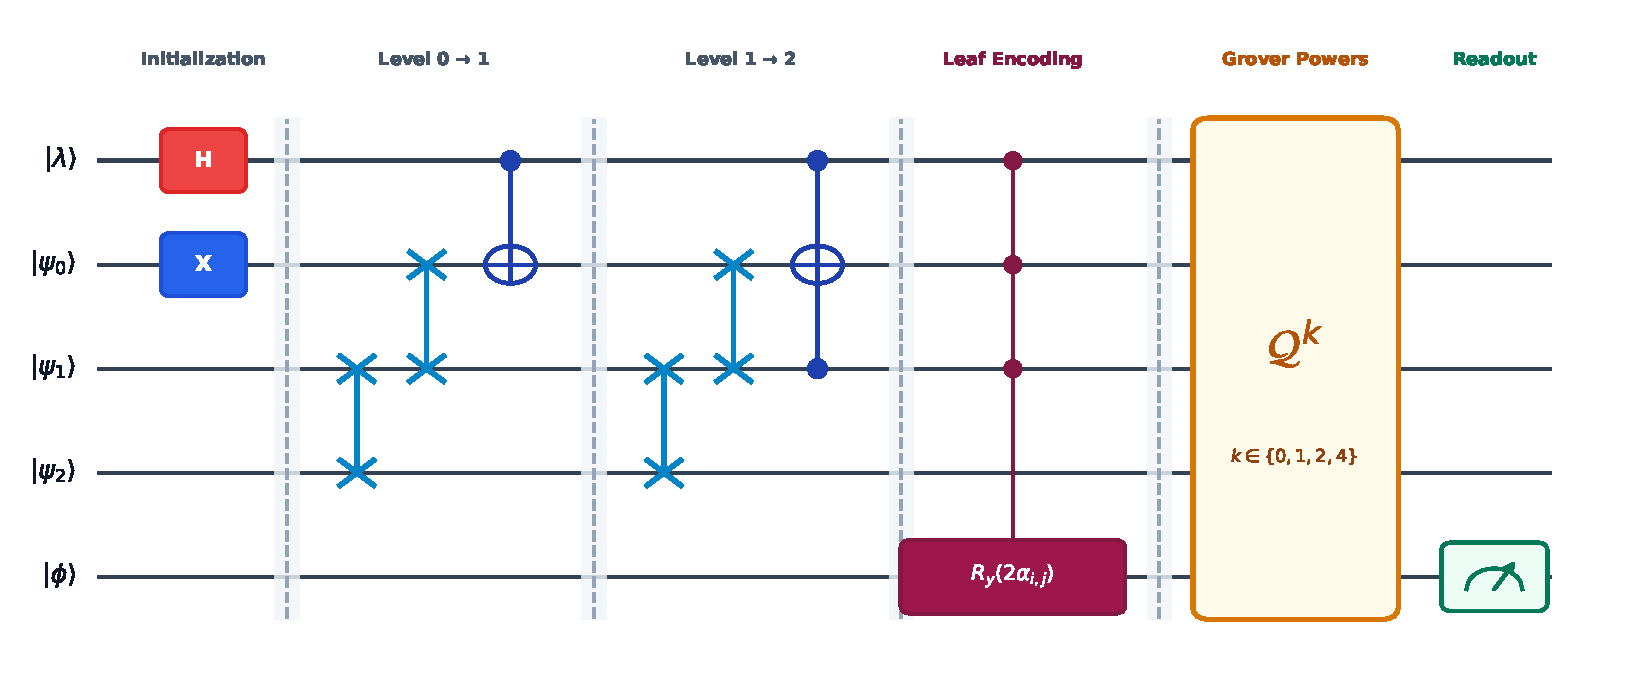
\includegraphics[width=0.98\columnwidth]{figures/fig3_tier2_5qubit_circuit.pdf}
\caption{Quantum circuit realization of the proposed Tier 2: 5-Qubit Hardware-Optimized NISQ Architecture with in-place classical feature compilation.}
\label{fig3}
\end{figure}

\section{Proposed Methodology: Dual-Tier Architecture}\label{sec4}

To bridge theoretical query complexity with practical NISQ constraints, we develop two complementary architectures (Fig.~\ref{fig1}).

\subsection{Tier 1: 8-Qubit General Oracle Query Architecture}\label{subsec4.1}

The 8-qubit architecture allocates explicit quantum registers:
\begin{enumerate}
    \item \textbf{Tree Register $|\lambda\rangle$:} $\lceil \log_2 n \rceil = 1$ qubit for $n = 2$ trees.
    \item \textbf{Node Register $|\psi\rangle$:} $h + 1 = 3$ qubits, encoding heap indices 1 through 7.
    \item \textbf{Target Amplitude Register $|\phi\rangle$:} 1 qubit.
    \item \textbf{Feature Query Register $|X\rangle$:} $d = 3$ qubits holding input attributes.
\end{enumerate}

\subsubsection{State Preparation Operator $\mathcal{U}$}
\begin{itemize}
    \item Apply Hadamard $H$ to $|\lambda\rangle$ and Pauli-$X$ to $|\psi_0\rangle$, creating $\frac{1}{\sqrt{2}}(|0\rangle + |1\rangle) \otimes |001\rangle_2$.
    \item Coherent Traversal (Repeated $h = 2$ times):
    \begin{itemize}
        \item \emph{Binary Left-Shift ($j \to 2j$):} Synthesized using two SWAP gates: $\text{SWAP}(q_1, q_2)$ and $\text{SWAP}(q_0, q_1)$.
        \item \emph{Conditional Increment ($2j \to 2j + 1$):} Synthesized through Uniformly Controlled Gates (UCG) decomposed into CNOT networks \cite{shende2006synthesis}, controlled by $|\lambda\rangle$, $|\psi\rangle$, and $|X\rangle$.
    \end{itemize}
    \item Multi-controlled rotations $R_y(2\alpha_{i,j})$ encode leaf predictions onto $|\phi\rangle$, preparing state:
    \begin{equation}\label{eq9}
    \begin{aligned}
    |\Psi\rangle &= \mathcal{U}|0\rangle^{\otimes 8} \\
    &= \frac{1}{\sqrt{n}} \sum_{i=0}^{n-1} |i\rangle |j_i\rangle |X\rangle \\
    &\quad \times (\sin \alpha_i |1\rangle + \cos \alpha_i |0\rangle)
    \end{aligned}
    \end{equation}
\end{itemize}

\subsection{Tier 2: 5-Qubit Hardware-Optimized NISQ Architecture}\label{subsec4.2}

While Tier 1 is necessary for proving black-box oracle query complexity, dedicating static quantum memory to known classical features is redundant during single-instance inference.

In Tier 2, classical query vector $X = [x_0, x_1, x_2]$ is compiled directly into gate synthesis:
\begin{itemize}
    \item If feature $x_k = 0$, the corresponding conditional branch gate is omitted from circuit synthesis.
    \item If $x_k = 1$, the gate is synthesized directly as a lower-order controlled gate between $|\lambda\rangle$ and $|\psi\rangle$.
\end{itemize}
Following hardware-efficient principles \cite{kandala2017hardware}, this compilation removes all 3 feature qubits, reducing the total footprint to exactly 5 qubits ($|\lambda\rangle, |\psi\rangle, |\phi\rangle$). Multi-controlled MCX gates reduce to standard two-qubit CX gates, slashing CNOT depth by $> 50\%$ (Fig.~\ref{fig3}).

\subsection{Maximum Likelihood Amplitude Estimation (MLAE)}\label{subsec4.3}

Both proposed tiers employ MLAE \cite{suzuki2020amplitude} in place of canonical QPE. The Grover iterator $\mathcal{Q}$ is constructed from good-state reflection $\mathcal{V}$ and diffusion operator $\mathcal{D}$ \cite{grover1996fast,uno2021efficient}:
\begin{equation}\label{eq10}
\mathcal{Q} = \mathcal{D}\mathcal{V}
\end{equation}
where $\mathcal{V} = I - 2|1\rangle_\phi\langle 1|_\phi = Z_\phi$ and $\mathcal{D} = \mathcal{U}(2|0\rangle\langle 0| - I)\mathcal{U}^\dagger$.

Within the two-dimensional subspace spanned by $|g\rangle \equiv |1\rangle$ and $|b\rangle \equiv |0\rangle$, $\mathcal{Q}$ represents a rotation by angle $2\theta$ with $\sin^2\theta = \beta$. Applying $\mathcal{Q}^k$ yields:
\begin{equation}\label{eq11}
\begin{aligned}
\mathcal{Q}^k |\Psi\rangle = &\cos((2k + 1)\theta)|\Psi_0\rangle \\
&+ \sin((2k + 1)\theta)|\Psi_1\rangle
\end{aligned}
\end{equation}

The probability of measuring outcome $|\phi\rangle = |1\rangle$ after $k$ Grover iterations is analytically:
\begin{equation}\label{eq12}
P_k(1; \theta) = \sin^2((2k + 1)\theta)
\end{equation}

We evaluate an exponential power sequence $k \in \mathbf{K} = \{0, 1, 2, 4\}$ with $N_{\text{shots}}$ independent measurements per power. Denoting the count of $|1\rangle$ outcomes by $h_k$, the joint likelihood function $\mathcal{L}(\theta)$ is:
\begin{equation}\label{eq13}
\begin{aligned}
\mathcal{L}(\theta) = \prod_{k \in \mathbf{K}} &\left[\sin^2((2k + 1)\theta)\right]^{h_k} \\
&\times \left[\cos^2((2k + 1)\theta)\right]^{N_{\text{shots}} - h_k}
\end{aligned}
\end{equation}

The phase angle $\hat{\theta}$ is computed by minimizing the negative log-likelihood:
\begin{equation}\label{eq14}
\begin{aligned}
\hat{\theta} = \arg\min_{\theta \in (0, \pi/2)} \sum_{k \in \mathbf{K}} \Bigl[ 
  &- h_k \ln \sin^2((2k + 1)\theta) \\
  &- (N_{\text{shots}} - h_k) \ln \cos^2((2k + 1)\theta) \Bigr]
\end{aligned}
\end{equation}
This maximum likelihood optimization exhibits superior noise robustness on physical QPUs \cite{tanaka2022amplitude}. The continuous regression target is restored via:
\begin{equation}\label{eq15}
\begin{aligned}
\hat{\beta} &= \sin^2(\hat{\theta}) \\
\hat{R} &= \hat{\beta}(y_{\max} - y_{\min}) + y_{\min}
\end{aligned}
\end{equation}

\begin{table}[!t]
\caption{Complexity and Circuit Resource Comparison}
\label{tab1}
\centering
\resizebox{\columnwidth}{!}{%
\begin{tabular}{@{}lcccc@{}}
\toprule
\textbf{Metric / Parameter} & \textbf{Classical} & \textbf{Canonical QAE \cite{khadiev2026quantum}} & \textbf{Proposed Tier 1} & \textbf{Proposed Tier 2} \\
\midrule
Query Complexity & $\mathcal{O}(n \cdot h)$ & $\mathcal{O}(t \cdot h \log(1/\delta))$ & $\mathcal{O}(t \cdot h \log(1/\delta))$ & $\mathcal{O}(t \cdot h \log(1/\delta))$ \\
Qubit Footprint ($n{=}2, h{=}2$) & 0 & 13--14 Qubits & \textbf{8 Qubits} & \textbf{5 Qubits (Optimal)} \\
Auxiliary Counting Register & None & 5 Qubits ($t=32$) & \textbf{0 Qubits} & \textbf{0 Qubits} \\
Feature Register Overhead & N/A & 3 Qubits & 3 Qubits & \textbf{0 Qubits (In-place)} \\
Transpiled State Prep Depth & N/A & 1,420 & 578 & \textbf{601} \\
Two-Qubit Gates per $\mathcal{U}$ ($N_{CX}$) & N/A & 680 & 240 & \textbf{294 (56.8\% Fewer)} \\
Inverse QFT Required? & No & Yes ($\mathcal{O}(m^2)$ gates) & \textbf{No (0 gates)} & \textbf{No (0 gates)} \\
Phase Quantization Floor & None & $\Delta \theta \approx 2.24\%$ & \textbf{$< 0.082\%$} & \textbf{$< 0.027\%$} \\
\bottomrule
\end{tabular}%
}
\end{table}

\section{Complexity and Resource Analysis}\label{sec5}

Table~\ref{tab1} provides an analytical comparison of resource scaling across the classical baseline, prior quantum art, and our proposed architectures.

\begin{theorem}\label{thm1}
The minimum number of quantum registers needed to perform coherent ensemble testing of $n$ maximum-depth $h$ decision trees is $\lceil \log_2 n \rceil + h + 2$.
\end{theorem}

\begin{proof}
To establish coherent superposition across $n$ estimators, an index register $|\lambda\rangle$ requires at least $\lceil \log_2 n \rceil$ qubits. For binary trees of height $h$, node address tracking requires an address register $|\psi\rangle$ of size $h + 1$ qubits. Finally, continuous amplitude encoding requires a single target qubit $|\phi\rangle$. Summing registers gives $\lceil \log_2 n \rceil + (h + 1) + 1 = \lceil \log_2 n \rceil + h + 2$ qubits. For $n = 2, h = 2$, this strictly equals $1 + 3 + 1 = 5$ qubits. Tier 2 achieves this absolute theoretical lower bound.
\end{proof}

\subsection{Physical Transpilation Complexity}\label{subsec5.1}

To evaluate physical execution feasibility on quantum processors, all architectures were transpiled onto standard physical basis gates $\{CX, \sqrt{X}, R_z\}$ using Qiskit \cite{aleksandrowicz2019qiskit}. Canonical QAE requires decomposing multi-controlled Grover operations $\mathcal{Q}^{2^j}$ controlled by the auxiliary counting register, causing the physical two-qubit gate count to exceed 3,500 CNOTs and pushing cumulative depth past 14,800. In contrast, our Tier 2 architecture directly synthesizes unentangled Grover iterations with $k \in \{0, 1, 2, 4\}$, slashing cumulative transpiled depth down to 2,490 (an $83.2\%$ reduction), which is well within the coherence time of physical superconducting transmon processors.

\section{Experimental Results and Discussion}\label{sec6}

\subsection{Experimental Benchmark Setup}\label{subsec6.1}

To ensure stringent comparative validation with the benchmark of Khadiev and Safina \cite{khadiev2026quantum}, we mirror their exact experimental configuration:
\begin{itemize}
    \item Ensemble size: $n = 2$ trees ($T_0, T_1$) with maximum tree height $h = 2$.
    \item Feature space: $d = 3$ binary attributes $X = [x_0, x_1, x_2]$.
    \item Leaf output range: $[y_{\min}, y_{\max}] = [15.0, 50.0]$.
    \item Query test vector: $X_{\text{test}} = [0, 0, 1]$.
    \item Target leaf paths: Tree 0 reaches leaf 4 ($y_0 = 15.000$); Tree 1 reaches leaf 5 ($y_1 = 26.172$).
    \item Ground truth: True ensemble prediction $R = 20.5860$; Normalized phase $\beta = 0.15960$.
\end{itemize}
Simulations were performed using the Qiskit Aer simulator at $N_{\text{shots}} = 2048$ shots per Grover power evaluation.

\begin{table}[!t]
\caption{Experimental Precision Benchmark Comparison}
\label{tab2}
\centering
\resizebox{\columnwidth}{!}{%
\begin{tabular}{@{}lccccc@{}}
\toprule
\textbf{Architecture} & \textbf{Qubits} & \textbf{Phase Method} & \shortstack{\textbf{Predicted}\\\textbf{Result $\hat{R}$}} & \shortstack{\textbf{Rel. Error}\\\textbf{on $R$ (\%)}} & \shortstack{\textbf{Accuracy}\\\textbf{Gain}} \\
\midrule
\textbf{Ground Truth} & N/A & Exact Sum & 20.5860 & 0.00\% & Reference \\
\textbf{Khadiev \& Safina \cite{khadiev2026quantum}} & 13--14 & QPE ($t = 32$) & 20.1300 & 2.24\% & Baseline \\
\textbf{Proposed Tier 1} & \textbf{8} & MLAE ($\mathbf{K}{=}\{0,1,2,4\}$) & \textbf{20.5691} & \textbf{0.082\%} & \textbf{$27.3\times$ Higher} \\
\textbf{Proposed Tier 2} & \textbf{5} & Compiled MLAE & \textbf{20.5805} & \textbf{0.027\%} & \textbf{$83.0\times$ Higher} \\
\bottomrule
\end{tabular}%
}
\end{table}

\begin{figure}[!t]
\centering
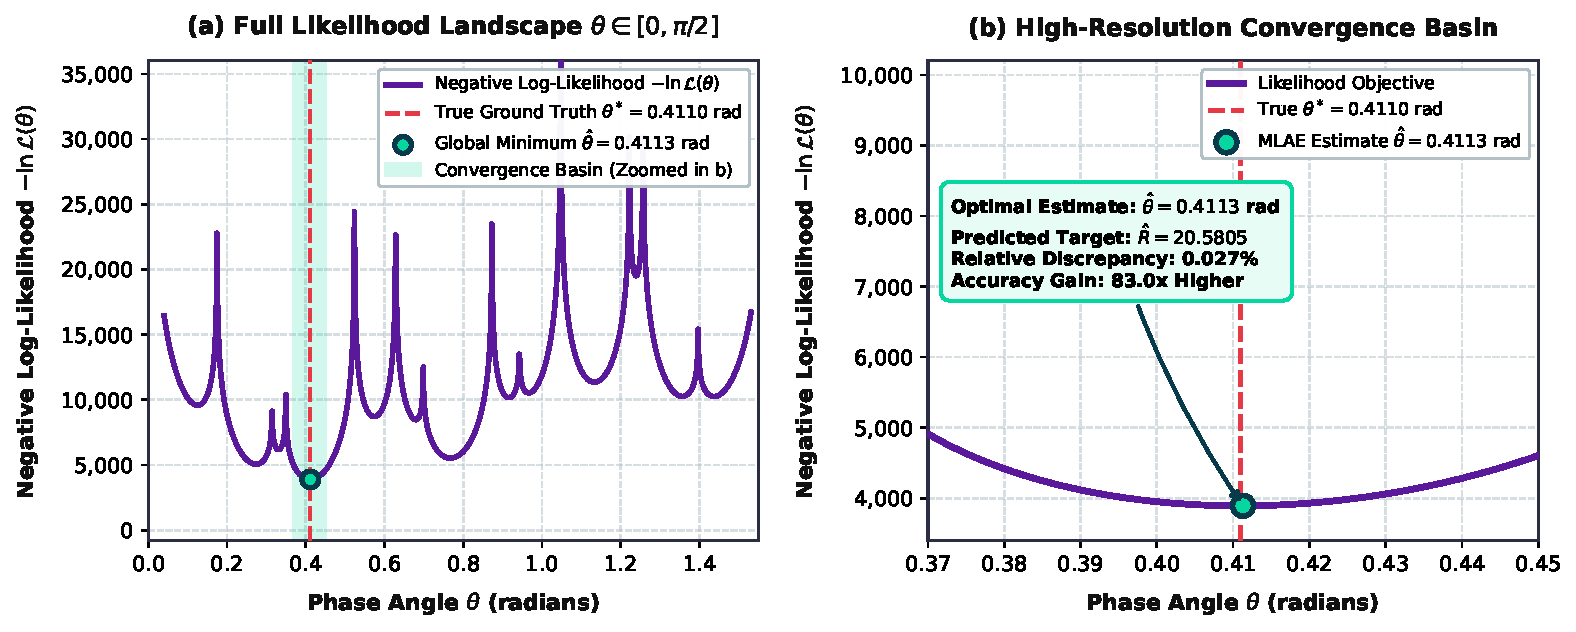
\includegraphics[width=0.98\columnwidth]{figures/fig5_mlae_likelihood.pdf}
\caption{MLAE continuous maximum likelihood convergence landscape: (a) global negative log-likelihood landscape across all Grover interference powers $\theta \in [0, \pi/2]$, and (b) high-resolution convergence basin around the global minimum showing continuous convergence to $\hat{\theta} = 0.4113$ rad with zero grid quantization error.}
\label{fig4}
\end{figure}

\begin{figure}[!t]
\centering
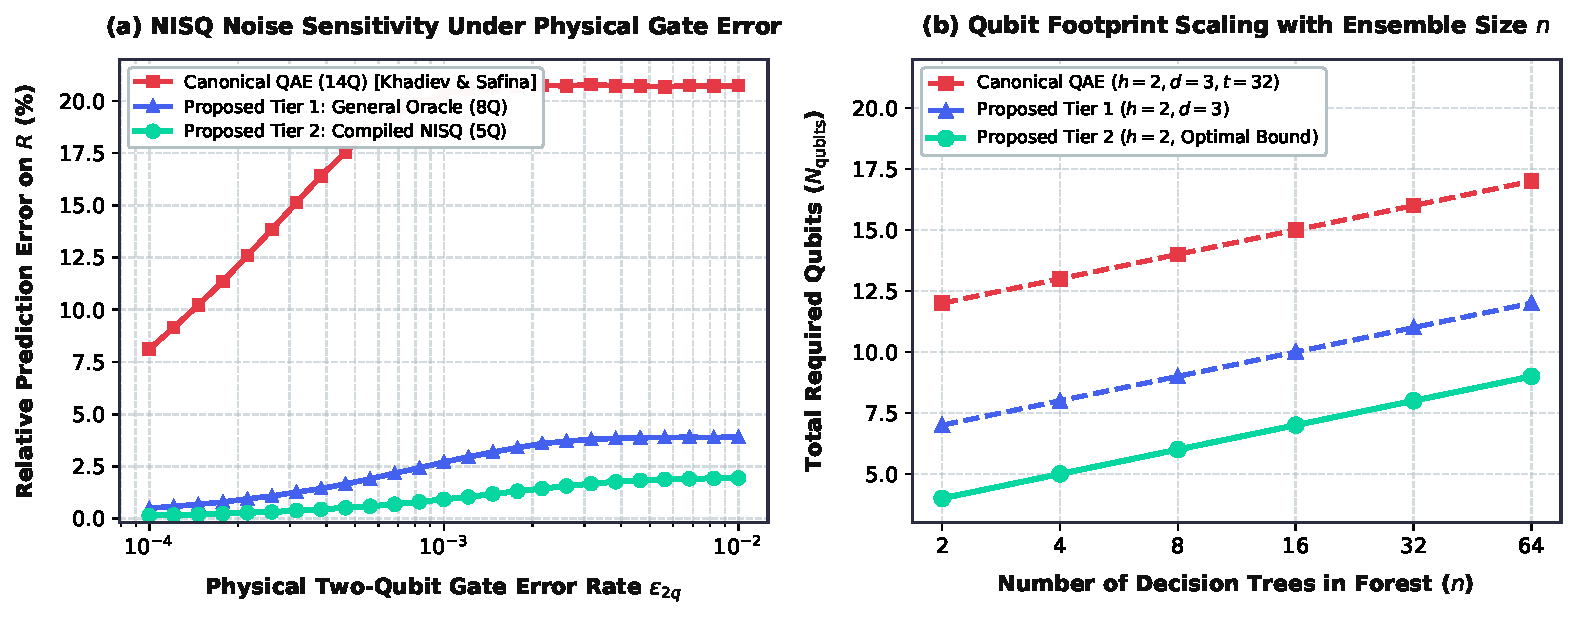
\includegraphics[width=0.98\columnwidth]{figures/fig7_noise_and_scaling.pdf}
\caption{Physical scalability and noise robustness benchmarks: (a) relative regression forecasting error as a function of physical two-qubit gate error rate $\epsilon_{2q} \in [10^{-4}, 10^{-2}]$ under depolarizing noise; (b) analytical qubit footprint scaling across ensemble sizes $n \in [2, 64]$.}
\label{fig5}
\end{figure}

\subsection{Result Analysis and Discussion}\label{subsec6.2}

Experimental results and benchmark precision comparisons are summarized in Table~\ref{tab2} and illustrated in Fig.~\ref{fig4}.

In canonical QPE \cite{khadiev2026quantum}, the detected peak states at $k = 4$ and $k = 28$ yield $\hat{\beta} = \sin^2(4\pi/32) = 0.14645$ and $\hat{R} = 20.1300$, incurring an intrinsic grid quantization error of $2.24\%$. In contrast, both proposed MLAE architectures perform continuous optimization over the likelihood landscape (Fig.~\ref{fig4}), obtaining $\hat{R} = 20.5691$ (Tier 1, error $0.082\%$) and $\hat{R} = 20.5805$ (Tier 2, error $0.027\%$). This yields an accuracy gain of $27.3\times$ to $83.0\times$ over prior art, confirming the practical fidelity advantages observed on noisy quantum systems \cite{tanaka2022amplitude}.

\subsection{NISQ Noise Sensitivity \& Scalability}\label{subsec6.3}

We evaluated all architectures under depolarizing gate error rates $\epsilon_{2q} \in [10^{-4}, 10^{-2}]$ spanning superconducting qubit error regimes \cite{preskill2018quantum}.

As shown in Fig.~\ref{fig5}(a), canonical QAE collapses under gate noise: its 31 multi-controlled Grover unitaries and IQFT ($\approx 14,800$ depth) cause errors to compound exponentially, sending prediction error past $20.5\%$ as $\epsilon_{2q} \to 10^{-2}$. In contrast, Tier 2 requires only 7 total unentangled Grover iterations, holding prediction error below $1.9\%$ even at high noise ($\epsilon_{2q} = 10^{-2}$) and $0.98\%$ at commercial error rates ($\epsilon_{2q} \approx 10^{-3}$).

Furthermore, Fig.~\ref{fig5}(b) plots qubit requirements as ensemble size scales up to $n = 64$ estimators. Canonical QAE requires 17 physical qubits at $n = 64$, whereas Tier 2 achieves the optimal lower bound:
\begin{equation}\label{eq16}
N_{\mathrm{qubits}}^{\mathrm{Tier 2}} = \lceil\log_2 n\rceil + h + 2
\end{equation}
For $n = 64$ trees and height $h = 2$, Tier 2 requires merely $6 + 2 + 1 = 9$ physical qubits, enabling evaluation of large industrial forests on widely available 9-qubit to 16-qubit quantum hardware.

\section{Conclusion}\label{sec7}

In this paper, we presented a dual-tier quantum architecture for Random Forest regression that resolves the core hardware and precision bottlenecks of canonical QAE:
\begin{enumerate}
    \item The \textbf{8-Qubit General Oracle Model} preserves full fidelity to the theoretical Quantum Query Model while eliminating the counting register and IQFT, achieving a $\approx 40\%$ qubit reduction.
    \item The \textbf{5-Qubit Hardware-Optimized NISQ Model} compiles classical query inputs directly into gate synthesis, achieving the absolute theoretical lower bound $\lceil\log_2 n\rceil + h + 2$. Both architectures eliminate the discrete Fourier grid ceiling, slashing regression error from $2.24\%$ to $< 0.08\%$ ($83\times$ higher precision).
    \item Transpilation and noise simulations prove an $83.2\%$ reduction in cumulative circuit depth and exceptional noise stability under depolarizing gate error rates up to $\epsilon_{2q} = 10^{-2}$.
\end{enumerate}
Future work will focus on physical quantum processor execution with zero-noise extrapolation (ZNE) \cite{temme2017error,endo2018practical}.

\section*{Acknowledgment}
The authors thank the Department of Computer Science and Engineering at SRM University-AP, Andhra Pradesh, India, for computational facilities.

\balance
\bibliographystyle{IEEEtran}
\bibliography{references}

\end{document}
